\chapter{Architecture}

 This chapter describes the architecture of the proposed corruption detection system. First, the Rust library developed specifically for this project is introduced, designed to operate efficiently both at the folder level and on individual data items. Then, the organization of the Merkle tree within the system is discussed, including how the agents (also referred to as \textit{nodes}) exchange information through the Raft cluster. Particular attention is given to scenarios in which some agents are temporarily unavailable (during uploads or during corruption checks) and how the system leverages the Raft log to maintain a consistent view of per-agent root hashes. This ensures that corruption verification can proceed safely and correctly, even when some agents lag behind or remain offline, independently of the Reed-Solomon requirement.

\section{Merkle Tree Library} \label{sec:merkle-tree-library}

As discussed in Section \ref{section:merkle-trees}, the integrity verification
protocol relies fundamentally on the Merkle tree data structure. Despite the widespread use of Merkle trees in the literature and in applications such as blockchains, there are relatively few general-purpose and reusable libraries available online. This is largely because implementations are often developed \textit{ad hoc}, tailored to the needs of a specific infrastructure or application domain.

To overcome this limitation, a dedicated library was developed in Rust\footnote{\url{https://www.rust-lang.org}}, named \texttt{mt-rs}. The library is distributed under a BSD-3 Licence on Crates.io\footnote{\url{https://crates.io/crates/mt-rs}}, with its source code publicly available at \url{https://github.com/boozec/mt}.

\paragraph{Hasher}

The construction of a Merkle tree begins with the definition of a \textit{hasher}, i.e., the cryptographic hash function applied to the leaves and internal nodes of the tree. This enables direct experimentation with different trade-offs between performance and security. The design allows developers to implement custom hashers by instantiating the trait \texttt{Hasher}, which requires only the implementation of the \texttt{hash} method. Listing \ref{code:hasher-example} illustrates a simple example of a user-defined hasher.


\begin{listing}[!ht]
\caption{Example of a custom hasher \texttt{FooHasher}, which hashes an input as a string with the prefix "foo\_" followed by the sum of the integer values of its bytes, in hexadecimal format.}
\label{code:hasher-example}
\begin{minted}[linenos,fontsize=\footnotesize]{Rust}
use mt_rs::hasher::Hasher;

pub struct FooHasher;

impl Hasher for FooHasher {
    fn hash(&self, input: &[u8]) -> String {
        let sum: u32 = input.iter().map(|&b| b as u32).sum();
        format!("foo_{:x}", sum)
    }
}
\end{minted}
\end{listing}


The library provides three default hashers: \texttt{SHA256Hasher}, \texttt{Keccak256Hasher}, and \texttt{Blake3Hasher}. They correspond to the functions analyzed in Section \ref{sec:cryptopgrahic-hash-functions}. 

\paragraph{Tree construction}
A Merkle tree is represented by the structure shown in Listing \ref{code:struct_merkletree}. It can be instantiated either from raw in-memory data using the \texttt{new} method or from the contents of files and folders using the \texttt{from\_paths} method (Listing \ref{code:new_and_from_paths_prototypes}). This dual approach supports both synthetic testing and real-world scenarios, such as integrity verification of storage systems, by avoiding repeated disk reads.

\begin{listing}[!ht]
\caption{\texttt{MerkleTree} structure definition, where \texttt{Node} is an ad hoc structure that includes additional information and methods.}
\label{code:struct_merkletree}
\begin{minted}[linenos,fontsize=\footnotesize]{Rust}
pub struct MerkleTree {
    /// Leaf nodes at the base of the tree 
    /// (may include a duplicate for even pairing).
    leaves: Vec<Node>,
    /// Height of the tree (number of levels including root).
    height: usize,
    /// Root node of the Merkle tree.
    root: Node,
}
\end{minted}
\end{listing}


\begin{listing}[H]
\caption{Signatures of the \texttt{new} and \texttt{from\_paths} methods. A concrete \texttt{Hasher} is always provided when defining a Merkle tree.}
\label{code:new_and_from_paths_prototypes}
\begin{minted}[linenos,fontsize=\footnotesize]{Rust}
impl MerkleTree {
    pub fn new<I, T, H>(hasher: H, data: I) -> Self
    where
        I: IntoIterator<Item = T>,
        T: AsRef<[u8]>,
        H: Hasher + 'static + std::marker::Sync,
    { /* ... */ }

    pub fn from_paths<H>(hasher: H, paths: Vec<String>) -> Self
    where
        H: Hasher + 'static + std::marker::Sync + Clone,
    { /* ... */ }
}
\end{minted}
\end{listing}

Internally, both methods translate the input data into leaf nodes of type \texttt{Node} and then invoke the builder function (Listing \ref{code:mt-build}), which assembles the tree level by level. The construction algorithm ensures binary balance by duplicating the last node when the number of nodes is odd.

Parallelization is achieved through the \texttt{par\_chunks} method of the Rayon crate\footnote{\url{https://crates.io/crates/rayon}}, which splits slices into disjoint chunks and computes parent nodes concurrently.

The tree is organized into \emph{levels}: the leaves at Level 1, the root at the highest level, and internal nodes in between (Figure \ref{fig:merkle-tree-levels}). This layered representation makes the structure conceptually simple. The root node is accessible through the \texttt{root()} method, and its hash can be retrieved directly. Unlike leaves and the root, internal nodes are not stored explicitly in the \texttt{MerkleTree} structure.

\begin{figure}[!ht]
\centering
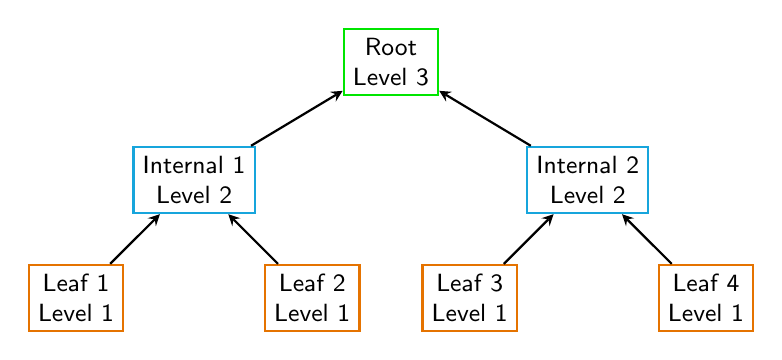
\begin{tikzpicture}[
  every node/.style={font=\sffamily\small, draw, rectangle, minimum size=8mm, align=center},
  greenborder/.style={draw=green!90!black, thick},
  blueborder/.style={draw=cyan!90!black, thick},
  yellowborder/.style={draw=orange!90!black, thick},
  level 1/.style={sibling distance=50mm, level distance=15mm},
  level 2/.style={sibling distance=30mm, level distance=15mm},
  level 3/.style={sibling distance=15mm, level distance=15mm},
  edge from parent/.style={draw, thick, <-, >=stealth}
]

% Root
\node[greenborder] {Root\\Level 3}
  child {node[blueborder] {Internal 1\\Level 2}
    child {node[yellowborder] {Leaf 1\\Level 1}}
    child {node[yellowborder] {Leaf 2\\Level 1}}
  }
  child {node[blueborder] {Internal 2\\Level 2}
    child {node[yellowborder] {Leaf 3\\Level 1}}
    child {node[yellowborder] {Leaf 4\\Level 1}}
  };

\end{tikzpicture}
\caption{An example of a binary Merkle tree with 4 leaves, showing the different levels: leaves (Level 1), internal nodes (Level 2), and the root (Level 3).}
\label{fig:merkle-tree-levels}
\end{figure}

\begin{listing}[H]
\caption{Build method for constructing the Merkle tree from the leaves upward. The \texttt{height} variable tracks the number of levels.}
\label{code:mt-build}
\begin{minted}[linenos,fontsize=\footnotesize]{Rust}
impl MerkleTree {
    fn build<H>(hasher: H, mut leaves: Vec<Node>) -> Self
    where
        H: Hasher + 'static + std::marker::Sync,
    {
        let original_leaves = leaves.clone();
        let mut height = 1;

        while leaves.len() > 1 {
            if leaves.len() % 2 != 0 {
                leaves.push(leaves.last().unwrap().clone());
            }

            leaves = leaves
                .par_chunks(2)
                .map(|pair| {
                    let combined = [
                        pair[0].hash().as_bytes(),
                        pair[1].hash().as_bytes()
                    ]
                    .concat();
                    
                    let hash = hasher.hash(&combined);
                    
                    Node::new_internal(hash, pair[0].clone(), pair[1].clone())
                })
                .collect();

            height += 1;
        }

        MerkleTree {
            leaves: original_leaves,
            height,
            root: leaves.into_iter().next().expect("root not found"),
        }
    }

}
\end{minted}
\end{listing}

Listing \ref{code:mt-root-print} demonstrates printing the Merkle tree root hash. The \texttt{hash()} method of each node returns the computed hash as a string.
\begin{listing}[H]
\caption{Snippet of code that prints the Merkle root hash of a tree with two byte strings as leaves.}
\label{code:mt-root-print}
\begin{minted}[linenos,fontsize=\footnotesize]{Rust}
let data = &["hello".as_bytes(), "world".as_bytes()];
let tree = MerkleTree::new(Blake3Hasher::new(), data);
println!("Merkle root: {}", tree.root().hash());
\end{minted}
\end{listing}

\paragraph{Proof generation and verification}
The library also supports Merkle proofs, which enable verification that a given leaf belongs to a specific Merkle tree. Proofs are generated and verified via implementations of the \texttt{Proofer} trait (Listing \ref{code:mt-proofer-trait}). A Merkle proof is expressed as sequences of \texttt{ProofNode} elements, which encode the sibling hashes encountered on the path from the leaf to the root. Users may define custom proofers if needed.

\begin{listing}[!htb]
\caption{The \texttt{Proofer} trait.}
\label{code:mt-proofer-trait}
\begin{minted}[linenos,fontsize=\footnotesize]{Rust}
/// Represents a single step in a Merkle proof path.
pub struct ProofNode {
    pub hash: String,
    pub child_type: NodeChildType, // Left or Right
}

/// A Merkle proof containing the path from a leaf to the root.
pub struct MerkleProof {
    pub path: Vec<ProofNode>,
    pub leaf_index: usize,
}

pub trait Proofer {
    /// Generates a Merkle proof for the data at the specified index
    fn generate(&self, index: usize) -> Option<MerkleProof>;

    /// Verifies that a piece of data exists in the tree using a Merkle proof
    fn verify<T>(&self, proof: &MerkleProof, data: T, root_hash: &str) -> bool
    where
        T: AsRef<[u8]>;
}
\end{minted}
\end{listing}


In this work, the \texttt{DefaultProofer} is used. Its implementation corresponds to proof generation (Algorithm \ref{algo:merkle-proof-generation}) and proof verification (Algorithm \ref{algo:merkle-proof-verification}). Unlike the \texttt{MerkleTree} structure, which does not store internal nodes, the \texttt{DefaultProofer} retains all levels.


Verification proceeds by iteratively reconstructing the root hash from the leaf and its authentication path, comparing the result with the expected root. The implementation in Rust is reported in Listing \ref{code:default-proofer}.

\begin{listing}[!htp]
\caption{Implementation of the \texttt{Proofer} trait for \texttt{DefaultProofer}. The proof is built by traversing the tree levels and collecting sibling hashes along the path.}
\label{code:default-proofer}
\begin{minted}[linenos,fontsize=\footnotesize]{Rust}
impl<H> Proofer for DefaultProofer<H>
where
    H: Hasher,
{
    fn generate(&self, index: usize) -> Option<MerkleProof> {
        if index >= self.levels[0].len() { return None; }
        let mut path = Vec::new();
        let mut current_index = index;
        for level in &self.levels[..self.levels.len() - 1] {
            let sibling_index = (current_index ^ 1).min(level.len() - 1);
            let sibling = &level[sibling_index];
            let child_type = if sibling_index < current_index {
                NodeChildType::Left
            } else {
                NodeChildType::Right
            };
            path.push(ProofNode {
                hash: sibling.hash().to_string(), child_type 
            });
            current_index >>= 1;
        }
        Some(MerkleProof { path, leaf_index: index })
    }

    fn verify<T>(&self, proof: &MerkleProof, data: T, root_hash: &str) -> bool
    where
        T: AsRef<[u8]>,
    {
        let mut current_hash = self.hasher.hash(data.as_ref());
        for proof_node in &proof.path {
            let combined: String = match proof_node.child_type {
                NodeChildType::Left => 
                    format!("{}{}", proof_node.hash, current_hash),
                NodeChildType::Right => 
                    format!("{}{}", current_hash, proof_node.hash),
            };
            current_hash = self.hasher.hash(combined.as_bytes());
        }
        current_hash == root_hash
    }
}
\end{minted}
\end{listing}

\newpage

\paragraph{Example and Conclusion}  
The complete workflow of the library is illustrated in Listing~\ref{code:mt-example}.
In this test, a Merkle tree is constructed from the folder \emph{pics}, which contains three files. The program verifies the basic properties of the tree, such as its height, and root hash, before generating a Merkle proof for the first leaf.  
Finally, the proof is successfully verified against the computed root hash, confirming the correctness of both tree construction and proofing. This example brings together the key components of the \texttt{mt-rs} library (hashers, tree building, and proof generation) and demonstrates their integration in practice, concluding the presentation of the Merkle tree library by showing how the system operates end-to-end on real data.


\begin{listing}[!htb]
\caption{End-to-end test of the \texttt{mt-rs} library: building a Merkle tree from the folder \emph{pics} (with three files), checking its properties, and verifying that a proof for the first leaf matches the expected root hash.}

\label{code:mt-example}
\begin{minted}[linenos,fontsize=\footnotesize]{Rust}
let hasher = Blake3Hasher::new();
let folders = vec![String::from("pics/")];

let tree = 
    MerkleTree::from_paths(hasher.clone(), folders);

assert_eq!(tree.height(), 3);
assert_eq!(
    tree.root().hash(),
    "a08c44656fb3f561619b8747a0d1dabe97126d9ed6e0cafbd7ce08ebe12d55ca"
);

let proofer = DefaultProofer::new(
    hasher.clone(), 
    // Recursively hashes the contents of files and directories.
    hash_dir(hasher.clone(), folders), 
);

let proof = proofer.generate(0).expect("proof generation failed");

assert!(proofer.verify(
    &proof,
    // Read the content of the first leaf read by the folder pics/
    &fs::read("pics/photo0.png").expect("file not found"),
    "a08c44656fb3f561619b8747a0d1dabe97126d9ed6e0cafbd7ce08ebe12d55ca"
));
\end{minted}
\end{listing}

\input{chapters/architecture/file-organisation}
\section{A Raft Cluster for File Uploads} \label{sec:raft-cluster-for-file-uploads}

In Section \ref{sec:raft}, the Raft consensus algorithm was introduced. This section explains its role within the proposed file corruption detection system, focusing on how Raft enables global agreement among agents on the Merkle root hashes associated with different folders.

As discussed in the previous section, there is no practical distinction between top-level and second-level folder roots: both are stored uniformly. The key requirement is that each agent must be aware of the Merkle root hash of every folder \emph{globally}, not just for its own local filesystem. This consistency is ensured through a Raft cluster, in which all agents act as nodes. Each node maintains a replicated log that functions as a command list of operations for a distributed key/value store, where folder identifiers serve as keys and the corresponding Merkle root hashes serve as values. Ideally, every correct node maintains an identical log, guaranteeing global agreement.

In practice, the Raft log is a sequence of messages broadcast by the leader to all nodes. Since the Raft cluster includes all agents, the terms \emph{node} and \emph{agent} can be used interchangeably. If an agent is online, it is part of the Raft cluster as well.

The log allows each agent to reconstruct "two levels" of a map, corresponding to the two levels of folder roots. Whenever a node restarts or rejoins the cluster, the log is replayed to restore state consistency. For example, in the scenarios illustrated in Figures \ref{fig:merkle-tree-first-level-of-saved-hashes} and \ref{fig:merkle-tree-second-level-of-saved-hashes}, each agent would maintain a single map such as:

\begin{listing}[H]
\caption{Example of a map of Merkle root hashes. Whether the key represents a top-level or second-level folder is irrelevant for now.}
\label{code:map-of-roots}
\begin{minted}[fontsize=\footnotesize]{Python}
roots = {
    # (1) Roots of top-level folders:
    "fe":   "root hash of fe",
    "ff":   "root hash of ff",
    
    # (2) Roots of second-level folders:
    "fe/2d":"root hash of fe/2d",
    "ff/4c":"root hash of ff/4c",
    "ff/6d":"root hash of ff/6d"
}
\end{minted}
\end{listing}

Only the Raft leader is allowed to append new messages to the log. In other words, one designated agent is responsible for broadcasting updates so that all other agents converge on the same global map.

Figure \ref{fig:sequence-diagram-upload-file} shows the sequence of events when a user uploads a file via the gateway (the service exposed for uploads and downloads). The gateway (GW) communicates directly with all agents, and the agents form a Raft cluster. Each action triggers local computations, and the figure illustrates how updates propagate through the system:

\renewcommand{\labelenumi}{\textbf{(\theenumi)}}
\begin{enumerate}
    \item The gateway receives a file, applies Reed-Solomon encoding, and splits it into $n+k$ shards. It generates a random salt (e.g., two bytes) and appends it to the filename (e.g., \texttt{photo.png24}). The salt prevents filename collisions and ensures randomized placement of the shards. Each shard is then sent to a different agent.
    \item Each agent uses a deterministic algorithm to transform the filename+salt into a unique hexadecimal identifier (e.g., \texttt{ff4c4b3}). This ensures the file is placed in a folder not previously used or marked as corrupted. The file is then stored under a two-level folder hierarchy (e.g., \texttt{ff/4c/4b3}). Each agent appends its identifier (i.e., \texttt{.1}, \texttt{.2}, \texttt{.3}) and saves the shard locally (e.g., \texttt{ff/4c/4b3.1} for Agent 1).
    \item Each agent computes the updated Merkle root hashes for the affected folders (e.g., \texttt{ff} and \texttt{ff/4c}) and sends them to the leader. Since any file modification propagates to the corresponding folder root, this step ensures consistency even when the top-level or second-level folders already contain files.
    \item The leader aggregates the roots received from all agents and computes global Merkle roots for each folder as illustrated in Figures \ref{fig:merkle-tree-first-level-of-saved-hashes} and \ref{fig:merkle-tree-second-level-of-saved-hashes} (e.g., one for \texttt{ff}, one for \texttt{ff/4c}). The leader appends these values to the Raft log, which is replicated across the cluster. 
\end{enumerate}

As a result, all agents maintain an up-to-date map from folder names to their latest root hashes, as illustrated in Listing \ref{code:map-of-roots}.

\setcounter{enumi}{0}

\begin{figure}[!ht]
\centering
\begin{tikzpicture}[scale=0.8, every node/.style={scale=0.8}]
\begin{umlseqdiag}
    % Define participants with more spacing
    \umlactor[no ddots, x=0]{User}
    \umlobject[no ddots, x=3]{GW}
    \umlobject[no ddots, x=7]{Agent 1}
    \umlobject[no ddots, x=11]{Agent 2}
    \umlobject[no ddots, x=15]{Agent 3}
    
    % Initial upload
    \begin{umlcall}[op=(1) Upload a file, return=, dt=10]{User}{GW}
    \end{umlcall}
    
    % GW to Agent 1
    \begin{umlcall}[op=(2a) Upload shard 1, dt=10]{GW}{Agent 1}
    \end{umlcall}
    
    % GW to Agent 2
    \begin{umlcall}[op=(2b) Upload shard 2, dt=10]{GW}{Agent 2}
    \end{umlcall}
    
    
    % GW to Agent 3
    \begin{umlcall}[op=(2c) Upload shard 3, dt=10]{GW}{Agent 3}
    \end{umlcall}
    
    % Agent 2 to Agent 1 - with spacing
    \begin{umlcall}[op=(3a) Root hashes of \texttt{ff} and \texttt{ff/4c}, dt=22]{Agent 2}{Agent 1}
    \end{umlcall}
    
    % Agent 3 to Agent 1 - with spacing
    \begin{umlcall}[op=(3b) Root hashes of \texttt{ff} and \texttt{ff/4c}, dt=22]{Agent 3}{Agent 1}
    \end{umlcall}
    
    % Self-call on Agent 1 - with spacing
    \begin{umlcall}[op=(3c) Root hashes of \texttt{ff} and \texttt{ff/4c}, dt=10]{Agent 1}{Agent 1}
    \end{umlcall}
    
    
    % Red arrows for Raft log distribution - with spacing
    \begin{umlcall}[op=(4a) Raft log with root hash for \texttt{ff} and \texttt{ff/4c}, fill=red, dt=10]{Agent 1}{Agent 2}
    \end{umlcall}
    
    \begin{umlcall}[op=(4b) Raft log with root hash for \texttt{ff} and \texttt{ff/4c}, fill=red, dt=10]{Agent 1}{Agent 3}
    \end{umlcall}
\end{umlseqdiag}
\end{tikzpicture}
\caption{Sequence diagram for uploading a file. In this example, Agent 1 is the Raft leader and the uploaded file has a path starting with \texttt{ff/4c}.}
\label{fig:sequence-diagram-upload-file}
\end{figure}

\newpage
\subsection{Corruption Check} \label{sec:check-corruption}

While Figure \ref{fig:sequence-diagram-upload-file} illustrates how uploads are handled, an equally important question remains: how can the system detect corrupted files? This is the purpose of the \emph{Corruption Check} process.

The process, executed at regular intervals for all top-level folders, is initiated by the leader. This responsibility lies with the leader because it is the only agent authorised to append new entries to the log. If corruption is detected, the leader records the result in the Raft log, thereby propagating the information consistently to all other agents.

Although earlier sections emphasized that top-level and second-level folders are stored uniformly, a practical distinction emerges during corruption checks. If a top-level folder is verified as intact, there is no need to check its subfolders. This follows from the Merkle tree property: any modification to a leaf propagates upward, changing the root. Thus, an unchanged top-level root implies that all second-level folders beneath it are also intact. Conversely, if a top-level folder's root does not match, the leader must recursively verify all second-level folders belonging to it.

In the best case, only the top-level folders need to be examined (a maximum of 256 keys, $16^2$). In the worst case, when every top-level folder fails verification, all second-level folders must also be checked (up to 65536 keys, $16^4$). This scenario corresponds to widespread corruption, where each top-level folder contains at least one corrupted file.

Figure \ref{fig:sequence-diagram-check-corruptions} illustrates the process for a top-level folder:

\renewcommand{\labelenumi}{\textbf{(\theenumi)}}
\begin{enumerate}
    \item The leader queries $n+k$ agents for the Merkle root hash of a given top-level folder (e.g., \texttt{ff}). It then applies the Merkle proof verification procedure, comparing the collected root hashes against the previously stored root (e.g. \texttt{roots["ff"]}).
    \item The leader appends the result of this verification to the Raft log, broadcasting whether the folder is corrupted. If the folder is marked as corrupted, the process is recursively repeated for all of its second-level subfolders (e.g. \texttt{ff/4c} and \texttt{ff/6d}).
\end{enumerate}

As a result, all agents share a consistent view of which folders are marked as corrupted. A top-level folder is corrupted if at least one of its subfolders is corrupted.

\begin{figure}[!ht]
\centering
\begin{tikzpicture}[scale=0.8, every node/.style={scale=0.8}]
\begin{umlseqdiag}
    % Define participants with more spacing
    \umlobject[no ddots, x=0]{Agent 1}
    \umlobject[no ddots, x=9]{Agent 2}
    \umlobject[no ddots, x=14]{Agent 3}

    \begin{umlcall}[op=(1a) Get root hash for \texttt{ff}, dt=10, return=Root hash for \texttt{ff}]{Agent 1}{Agent 1}
    \end{umlcall}
      
    \begin{umlcall}[op=(1b) Get root hash for \texttt{ff}, dt=10, return=Root hash for \texttt{ff}{Agent 1}{Agent 2}
    \end{umlcall}

    \begin{umlcall}[op=(1c) Get root hash for \texttt{ff}, dt=10, return=Root hash for \texttt{ff}]{Agent 1}{Agent 3}
    \end{umlcall}

    \begin{umlcall}[op=(2a) Raft log with corruption status for \texttt{ff}, fill=red, dt=10]{Agent 1}{Agent 2}
    \end{umlcall}
    \begin{umlcall}[op=(2b) Raft log with corruption status for \texttt{ff}, fill=red, dt=10]{Agent 1}{Agent 2}
    \end{umlcall}
\end{umlseqdiag}
\end{tikzpicture}
\caption{Sequence diagram illustrating the Corruption Check process for the top-level folder \texttt{ff}. Agent 1 is the Raft leader.}
\label{fig:sequence-diagram-check-corruptions}
\end{figure}

\subsection{Corruption Check for Partial Uploads}

The mechanisms described so far assumed that all agents are continuously online. In practice, temporary unavailability of agents is unavoidable. This subsection extends the model by considering two cases: (i) when an agent is offline during a file upload, and (ii) when one or more agents are offline during the corruption check itself.

To mitigate these cases, the data structures introduced in Listing \ref{code:map-of-roots} are extended. Instead of storing only a single Merkle root hash per folder (both top-level and second-level), the system also records Merkle root hashes for every agent. This results in two complementary maps:
\begin{itemize}
\item \textbf{roots}: a map from folder identifiers to global root hashes. Each value is the aggregated Merkle root computed over all agents' contributions for that folder.
\item \textbf{agent\_roots}: a map from folder identifiers to the set of per-agent root hashes. Each value explicitly tracks the current Merkle root hash for the corresponding folder, stored in an array indexed from $1$ to $n+k$.
\end{itemize}

If an agent was offline during an upload, its entry in the array remains empty for a new entry or unedited for an older one. Thanks to the Raft log, these per-agent arrays are consistently replicated across all agents. This ensures that even if a leader crashes and a new leader is elected, the corruption check phase remains unaffected.

An example is shown in Listing \ref{code:map-of-roots-2}, where Agent 3 was offline during certain uploads. In this case, some entries of the \texttt{roots} map are computed using only two leaves, since the third leaf in the corresponding \texttt{agent\_roots} entries is \texttt{nil}.

\begin{listing}[H]
\caption{Example of folder root hashes with $n=2$, $k=1$. Agent 3 was offline during the upload of files in \texttt{ff} folder.}
\label{code:map-of-roots-2}
\begin{minted}[fontsize=\footnotesize]{Python}
roots = {
    "fe":   "root hash of fe",
    "ff":   "root hash of ff",
    "fe/2d":"root hash of fe/2d",
    "ff/4c":"root hash of ff/4c",
    "ff/6d":"root hash of ff/6d"
}

agent_roots = {
    "fe":[
        "Agent 1 root hash of fe",
        "Agent 2 root hash of fe",
        "Agent 3 root hash of fe"
    ],
    "ff":["Agent 1 root hash of ff",   "Agent 2 root hash of ff",   nil],
    "fe/2d":[
        "Agent 1 root hash of fe/2d",
        "Agent 2 root hash of fe/2d",
        "Agent 3 root hash of fe/2d"
    ],
    "ff/4c":["Agent 1 root hash of ff/4c","Agent 2 root hash of ff/4c",nil],
    "ff/6d":["Agent 1 root hash of ff/6d","Agent 2 root hash of ff/6d",nil]
}
\end{minted}
\end{listing}

It is important to note that root hashes are stored at the \emph{folder} level, not per file. As a result, \texttt{agent\_roots[<some\_folder>]} may contain entries that are not perfectly aligned across agents. For example, Agents 1 and 2 may have already uploaded ten files into a folder, while Agent 3, having been offline, may only have one file in the same folder.  

This apparent asymmetry does not compromise correctness. The reason is that \texttt{roots[<some\_folder>]} is computed as a Merkle root over the entire array \texttt{agent\_roots[<some\_folder>]}. Even if one agent's contribution lags behind, the global root still represents a consistent snapshot of the folder state across all agents. During verification, the Merkle proof ensures that each agent's current hash (or stored historical hash, if offline) matches the position it contributed to in the global root.  

\paragraph{Agent offline during upload}

If an agent is offline during an upload, the system can still guarantee correctness as long as the Reed-Solomon requirement is satisfied. In an $n+k$ configuration, at least $n$ agents must be online, since $n$ shards are sufficient to reconstruct the file on download.

If an agent was offline during an upload, its entry in the per-agent array remains empty (or unedited). Thanks to the Raft log, these arrays are consistently replicated across all agents. Because the system does not modify the entry corresponding to the offline agent, the Merkle root computed in \texttt{roots} correctly reflects the full folder state, including the filesystem status of the offline agent. Therefore, the global Merkle root remains consistent even if some agents are temporarily unavailable.

When the offline agent later rejoins, it synchronizes its metadata by replaying the Raft log. However, it does not automatically reconstruct the shards it missed during downtime. During a corruption check, the leader queries the folder root hashes from all agents. For an agent that was previously offline, the stored value in \texttt{agent\_roots} is exactly what the leader expects. Thus, the check does not fail: the Merkle root returned by the previously offline agent is consistent with the snapshot that the leader uses for verification, assuming no corruption has occurred.

This reasoning naturally generalizes to the case where up to $k$ agents are offline at the same time: as long as at least $n$ agents remain available, the system continues to satisfy the Reed-Solomon requirement.

\paragraph{Agents offline during corruption check}

A more challenging scenario arises when some agents are offline during the corruption check itself. The set of agents currently online may differ from those that participated in the original upload. If the leader cannot collect the current Merkle root for a folder from all agents (even when some entries in \texttt{agent\_roots} are \texttt{nil}) the corruption check for that folder must rely on the available data. Consequently, the check process is adapted to handle offline agents gracefully.

During a corruption check for a folder, the leader iterates over all $n+k$ positions:  
\begin{itemize}
    \item If agent $i$ is online, it requests the current root hash from that agent.  
    \item If agent $i$ is offline, it retrieves the saved value from the corresponding slot in \texttt{agent\_roots}.  
\end{itemize}

Once all $n+k$ values are collected, the leader performs the Merkle proof verification against the global root hash stored in \texttt{roots}. This process is illustrated in Figure \ref{fig:flow-chart-check-corruption}.  

\begin{figure}[!htp]
\centering
\begin{tikzpicture}[node distance=2cm]

\tikzstyle{process} = [rectangle, minimum width=3cm, minimum height=1cm,
                       text centered, text width=3cm, draw=black]
\tikzstyle{decision} = [diamond, minimum width=3cm, minimum height=1cm,
                        text centered, draw=black]
\tikzstyle{arrow} = [thick,->,>=stealth]

\node (pro1) [process] {$i = 1$};
\node (dec1) [decision, below of=pro1, yshift=-1.5cm] {Is Agent $i$ online?};
\node (pro2a) [process, below of=dec1, yshift=-2cm] {Request current root hash from Agent $i$};
\node (pro2b) [process, right of=dec1, xshift=3cm, font=\small] {Retrieve saved root hash from \texttt{hashes["ff"][i]}};
\node (dec2) [decision, below of=pro2a, yshift=-1cm] {$i = n+k$?};
\node (pro3) [process, left of=dec2, xshift=-3cm] {$i = i+1$};
\node (pro4) [process, below of=dec2, yshift=-2cm] {Verify Merkle Tree Proof with collected hashes and \texttt{roots["ff"]}};

\draw [arrow] (pro1) -- (dec1);
\draw [arrow] (dec1) -- node[anchor=east] {yes} (pro2a);
\draw [arrow] (dec1) -- node[anchor=north] {no} (pro2b);
\draw [arrow] (pro2a) -- (dec2);
\draw [arrow] (pro2b) |- (dec2);
\draw [arrow] (dec2) -- node[anchor=north] {no} (pro3);
\draw [arrow] (pro3) |- (dec1);
\draw [arrow] (dec2) -- node[anchor=east] {yes} (pro4);

\end{tikzpicture}
\caption{Corruption check process for the top-level folder \texttt{ff}, considering some agents may be offline.}
\label{fig:flow-chart-check-corruption}
\end{figure}

Returning to the example: suppose Agent 2 goes offline while Agent 3 comes online. During the corruption check of folder \texttt{ff}, the system uses the stored value of Agent 2's root from \texttt{agent\_roots["ff"][2]}, while requesting a fresh root from Agent 3. If the Merkle proof verification succeeds, this guarantees that all currently online agents are consistent and uncorrupted. In this case, the status of offline agents is irrelevant:  
\begin{itemize}
    \item If the proof holds, online agents have uncorrupted data.
    \item If the proof fails, at least one online agent is corrupted, and the outcome is marked as a corruption regardless of the offline agents.  
\end{itemize}

This highlights an important distinction: the Corruption Check \ref{sec:check-corruption} phase itself does not rely on the Reed-Solomon requirement of having $n$ correct shards. Instead, it depends only on the fact that the Raft log ensures a consistent view of the per-agent root hashes across all agents. Offline agents may lag behind in state (or even remain offline for the entire process) without affecting the verification. In fact, it would be possible to perform the corruption check even if more than $k$ agents are offline. The correctness of the two cases considered (Agents offline during upload and Agents offline during the corruption check) is ensured because the first case already satisfies the Reed-Solomon reconstruction requirement, while the verification itself relies solely on the consistency guaranteed by Raft. Therefore, the corruption check can safely verify the folder state based on the available information, independently of the offline agents.

\subsection{Recovery of Missing Shards}

In the previous subsection, the reader learned what happens when an agent is offline during a file upload. This subsection discusses how missing shards are reconstructed when a previously offline agent comes back online.

The sequence diagram illustrated in Figure \ref{fig:sequence-diagram-upload-file} is simplified: every time a new shard is uploaded, the agent sends an acknowledgment to the leader. This allows the leader to maintain an up-to-date view of the cluster, tracking which agents are online and which have stored a shard for a given file, avoiding active pings or status checks. The acknowledgment is asynchronous, so the leader does not block waiting for responses. Meanwhile, the user receives confirmation through the gateway (GW), which handles shard uploads synchronously. In other words, shard storage and acknowledgment to the leader are independent processes.

Thanks to Raft, the leader keeps a log of all received acknowledgments. Recording this information in the Raft log ensures that every node in the cluster knows which agents were offline during the upload of a file. 

During the download process, some previously online agents might now be offline, and vice versa. Even if the set of online agents at upload time satisfied the Reed-Solomon requirement, there is no guarantee that the currently online agents hold enough shards (at least $n$) to reconstruct the file. When this happens, a recovery phase is necessary to restore the missing shards to ensure reconstruction.

Similar to the Corruption Check phase, a Recovery phase can be triggered to deliver missing shards to previously offline agents. The leader coordinates this process. To maintain consistency, the receiving agent recalculates the Merkle roots for both the top-level and second-level folders affected by the newly received shard. It then sends the updated roots back to the leader, which updates the corresponding $i$-th entries in \texttt{agent\_roots} and recomputes the global \texttt{roots} for the folders. Once the missing shard is successfully restored, the leader records the update in the Raft log to notify all nodes that the shard has been sent and the new values for the relevant \texttt{roots} and \texttt{agent\_roots} maps have been established.

Retaking the previous example shown in Listing \ref{code:map-of-roots-2}, after a full recovery all entries in \texttt{agent\_roots} are filled, as illustrated in Listing \ref{code:map-of-roots-3}.

\begin{listing}[H]
\caption{Example of folder root hashes with $n=2$, $k=1$ after every agent received all the shards.}
\label{code:map-of-roots-3}
\begin{minted}[fontsize=\footnotesize]{Python}
roots = {
    "fe":   "new root hash of fe",
    "ff":   "new root hash of ff",
    "fe/2d":"new root hash of fe/2d",
    "ff/4c":"new root hash of ff/4c",
    "ff/6d":"new root hash of ff/6d"
}

agent_roots = {
    "fe":   [
        "Agent 1 root hash of fe",
        "Agent 2 root hash of fe",
        "Agent 3 root hash of fe"
    ],
    # [...]
    "ff/6d":   [
        "Agent 1 root hash of ff/6d",
        "Agent 2 root hash of ff/6d",
        "Agent 3 root hash of ff/6d"
    ],
}
\end{minted}
\end{listing}

This chapter described how the Merkle tree solution was designed and integrated with a Raft cluster, explaining step by step how the main issues were addressed. The next chapter focuses on the implementation, presenting the developed solution and evaluating it through system-wide testing.